\subsection{Synonyms}

We have to remember that beyond n-gram frequency changes, there is also a shift in term of topics that are covered by newspapers over the years. To try to isolate our analysis from that effect, we planned to compare frequencies of words that have similar meaning using a synonym dictionary. After trying a few of them, we have chosen to use the myThes v2.0 synonym dictionary from OpenOffice that seemed exhaustive and accurate enough. \\

Frequency vectors were generated for every entry in the synonym database (using mapReduce) before being inserted in an SQL database. We have chosen to average frequencies to ranges of 5 years such as we limit the data size. Then we build a little web application that allows to check for words in the thesaurus database, then select a subset of the proposed similar words before displaying a plot with the evolution of frequencies.\\

This interactive application enabled us to quickly explore hypothesis we had about expected frequencies changes while, before, we needed to run a mapReduce job on the cluster for any chosen word. But most of the time, the synonyms proposed happen to have various meanings and were unsuitable to perform an automated analysis on our data. The intervention of the user was crucial during the selection phase to choose the appropriate ones. For instance a synonym for "voiture" (car) is "caisse" (slang) that also means box (by far its most frequent usage). Thus the perceived frequency of "caisse" will be strongly overstated and we cannot easily, at least for the scope of this project, tell apart the different meanings for a given 1-gram and split the occurrences accordingly.

\begin{figure}[H]
	\centering
        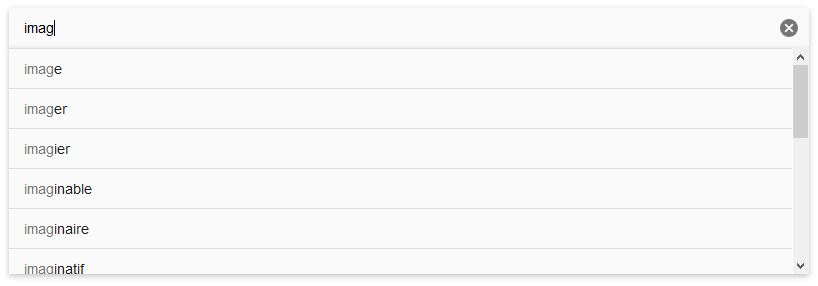
\includegraphics[scale=0.5]{Pictures/synonyms/search.jpeg}
        \caption{Seaching the thesaurus database with autocomplete}
        \label{search}
\end{figure}
\begin{figure}[H]
	\centering
        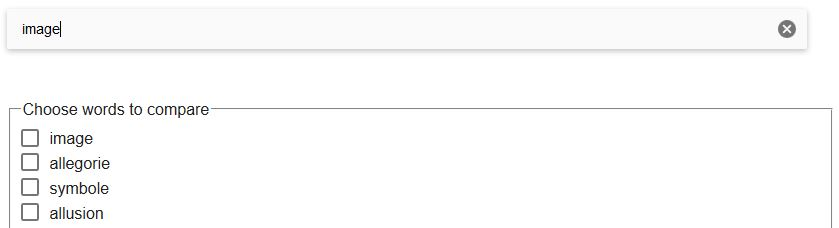
\includegraphics[scale=0.5]{Pictures/synonyms/select.jpeg}
        \caption{Check the proposed synonyms to display}
        \label{select}
\end{figure}

\begin{figure}[H]
	\centering
        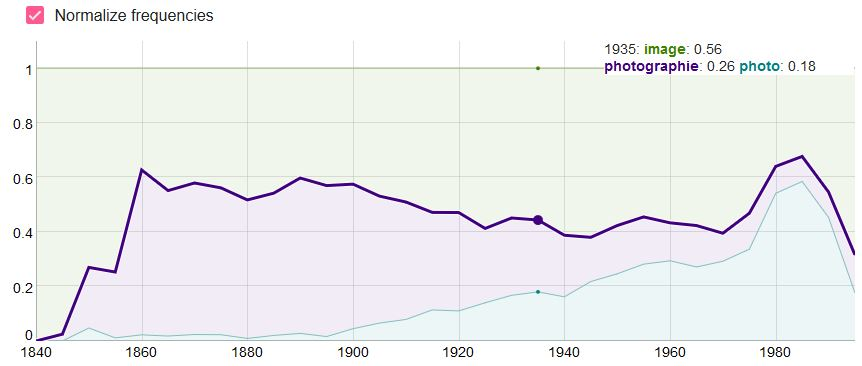
\includegraphics[scale=0.5]{Pictures/synonyms/graph.jpeg}
        \caption{Resulting frequency graph (with normalization option enabled)}
        \label{graph}
\end{figure}
